\begin{DoxyVersion}{Versión}
v1 
\end{DoxyVersion}
\begin{DoxyAuthor}{Autor}
Luis Baca, Óscar Gómez, Carmen Navarro y Carlos Cano
\end{DoxyAuthor}
\hypertarget{index_introduccion}{}\subsection{Introducción}\label{index_introduccion}
Los objetivos de este guión de prácticas son los siguientes\+:
\begin{DoxyItemize}
\item Resolver un problema eligiendo la mejor estructura de datos para las operaciones que se solicitan.
\end{DoxyItemize}

Los requisitos para poder realizar esta práctica son\+:
\begin{DoxyEnumerate}
\item Haber estudiado el Tema 1\+: Introducción a la eficiencia de los algoritmos
\item Haber estudiado el Tema 2\+: Abstracción de datos. Templates.
\item Haber estudiado el Tema 3\+: T.\+D.\+A. Lineales.
\item Haber estudiado el Tema 4\+: S\+TL e Iteradores.
\item Haber estudiado estructuras de datos jerárquicas\+: Árboles
\end{DoxyEnumerate}\hypertarget{index_objetivos}{}\subsection{Objetivos}\label{index_objetivos}
El objetivo de esta práctica es llevar a cabo el análisis, diseño e implementación de un proyecto. Con tal fin, el estudiante abordará un problema donde se requieren estructuras de datos que permiten almacenar grandes volúmenes de datos y poder acceder a ellos de la forma más eficiente.\hypertarget{index_problema}{}\subsection{Problema}\label{index_problema}
El estudiante debe implementar un programa que simule el juego \char`\"{}\+Conecta 4\char`\"{} \mbox{[}Conecta4\mbox{]}. El objetivo de Conecta 4 es alinear cuatro fichas sobre un tablero formado por seis filas y siete columnas. Cada jugador dispone de 21 fichas de un color (por lo general, rojas o amarillas). En nuestro caso, las fichas de los jugadores se indicarán con los caracteres \char`\"{}\+X\char`\"{} y \char`\"{}\+O\char`\"{}. Por turnos, los jugadores deben introducir una ficha en la columna que prefieran (siempre que no esté completa) y ésta caerá a la posición más baja. Gana la partida el primero que consiga alinear cuatro fichas consecutivas de un mismo color en horizontal, vertical o diagonal. Si todas las columnas están llenas pero nadie ha hecho una fila válida, hay empate.

El estudiante debe implementar una versión de este juego en el que los movimientos de uno de los jugadores se efectúan de forma automática. Esta modalidad, que llamaremos \char`\"{}\+Player V\+S. Computer\char`\"{} o \char`\"{}1 jugador automático\char`\"{}, requiere implementar un mecanismo de decisión automática basado en la disposición actual del tablero. Para implementar este mecanismo de decisión automática, debemos representar todos los posibles movimientos a partir del tablero actual y definir una \char`\"{}métrica\char`\"{} que nos permita \char`\"{}evaluar\char`\"{} cuál de los movimientos posibles deriva un tablero con más posibilidad de éxito para el jugador automático. Cuanto mejor sea esta métrica, más difícil será batir al jugador automático en una partida de Conecta 4.

Por ejemplo, la métrica más sencilla consistiría en evaluar si alguno de los movimientos posibles para el jugador automático produce directamente un tablero donde el jugador automático consigue 4 en línea (y, por tanto, gana la partida) o evita un 4 en línea del rival (y, por tanto, evita perder la partida). Sin embargo, esta métrica sólo nos permitiría evaluar ciertos tableros, dejándonos \char`\"{}a ciegas\char`\"{} para tomar una decisión en tableros que no derivan una victoria o derrota en un sólo movimiento. {\bfseries Otras métricas más sofisticadas requieren evaluar todos los posibles movimientos a partir de un tablero dado, contemplando varios turnos de los dos jugadores. Una representación natural para almacenar esta información es un Árbol}. El nodo raíz representa el tablero actual y le añadimos un hijo por cada posible tablero que se deriva del padre con un movimiento del jugador que tiene el turno. De este modo, el nivel 1 del árbol representa todos los movimientos posibles de uno de los jugadores, el nivel 2 todos movimientos posibles del otro jugador para cada uno de los tableros de nivel 1, y así sucesivamente. Cada rama del árbol termina en una hoja en la que, o bien se da la victoria de uno de los jugadores, o bien hay empate (no quedan movimientos posibles). Las siguientes figuras ilustran la estructura interna de un T\+DA Árbol General que almacena los tableros de Conecta 4 con la disposición de la partida en cada momento. La primera figura incide en la estructura interna del árbol y la segunda en posibles tableros almacenados en el árbol.


\begin{DoxyImage}
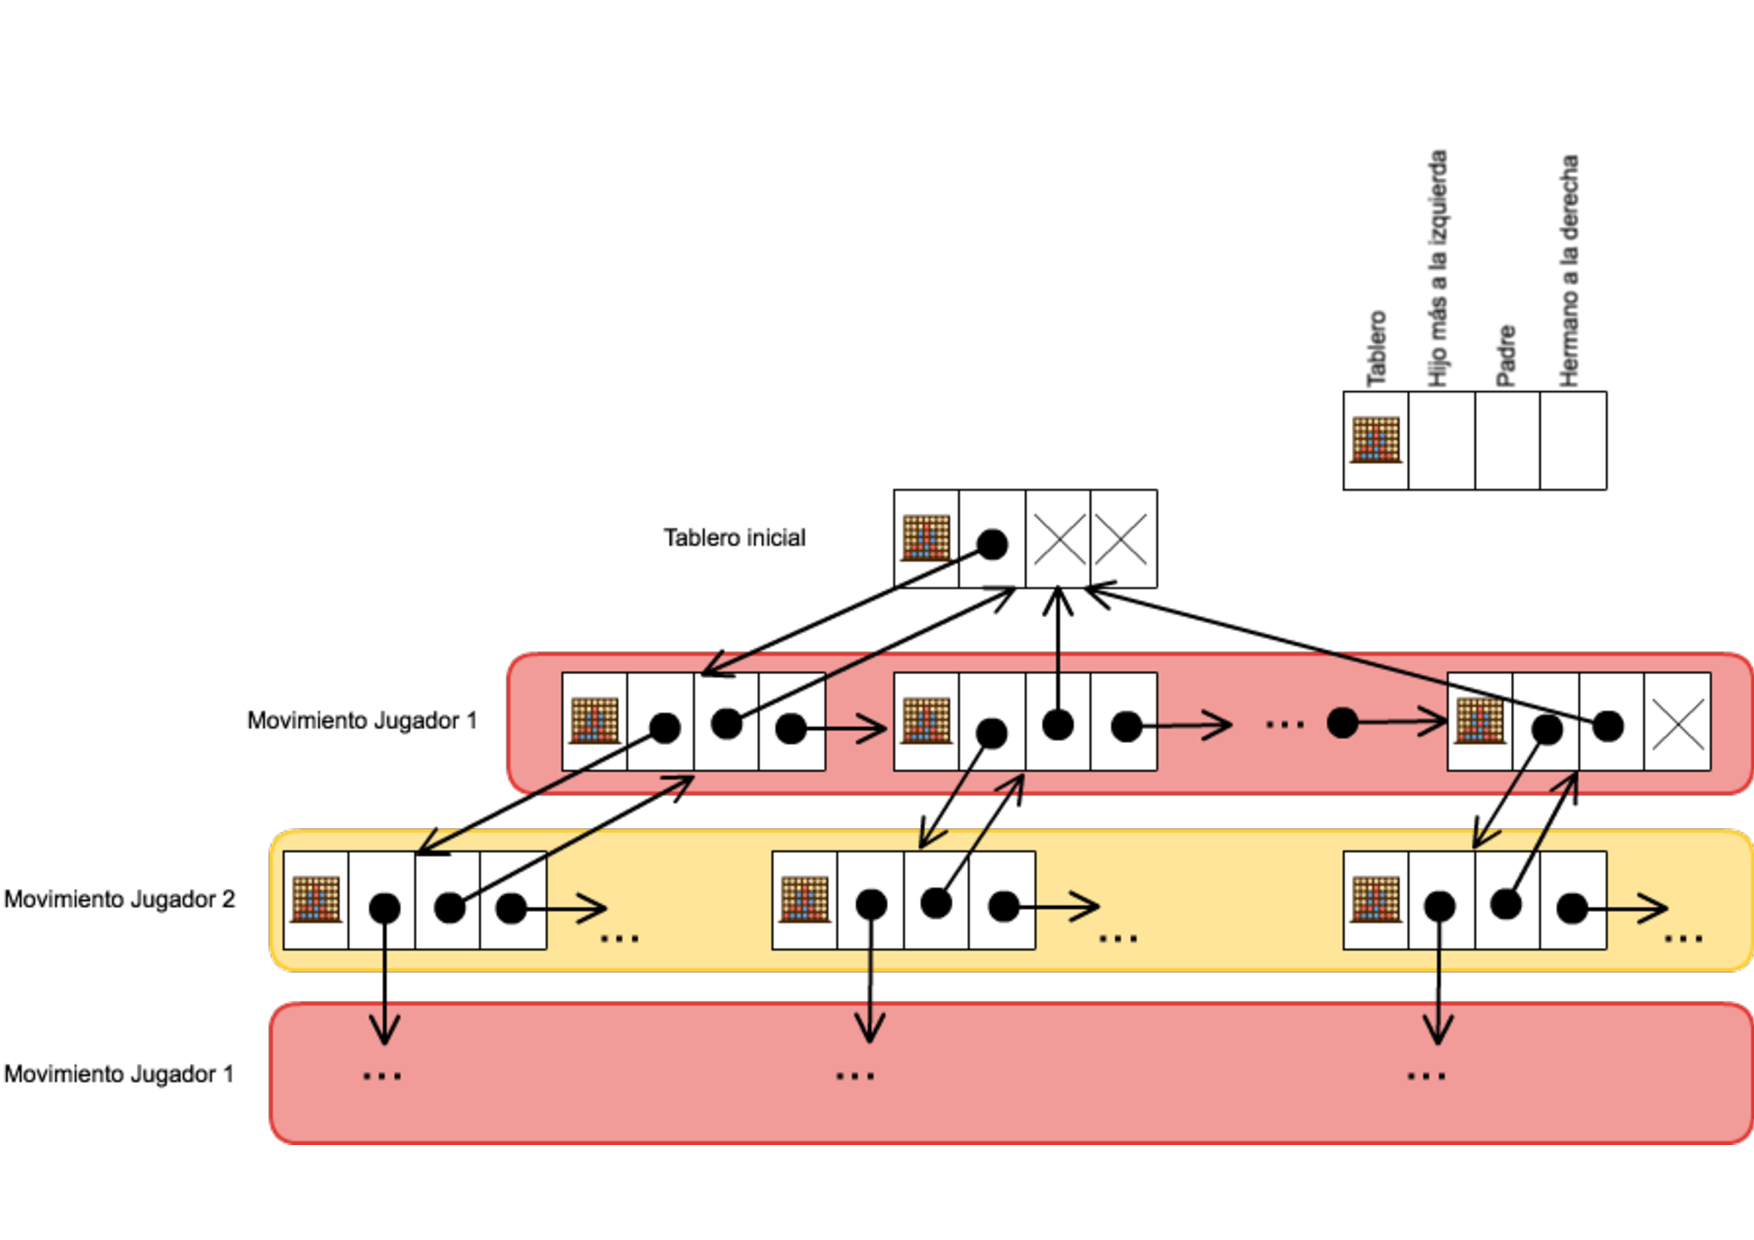
\includegraphics[width=12cm]{connect4-tree}
\caption{Estructura interna de un T\+DA Árbol General para representar el espacio de soluciones de Conecta 4}
\end{DoxyImage}







\begin{DoxyImage}
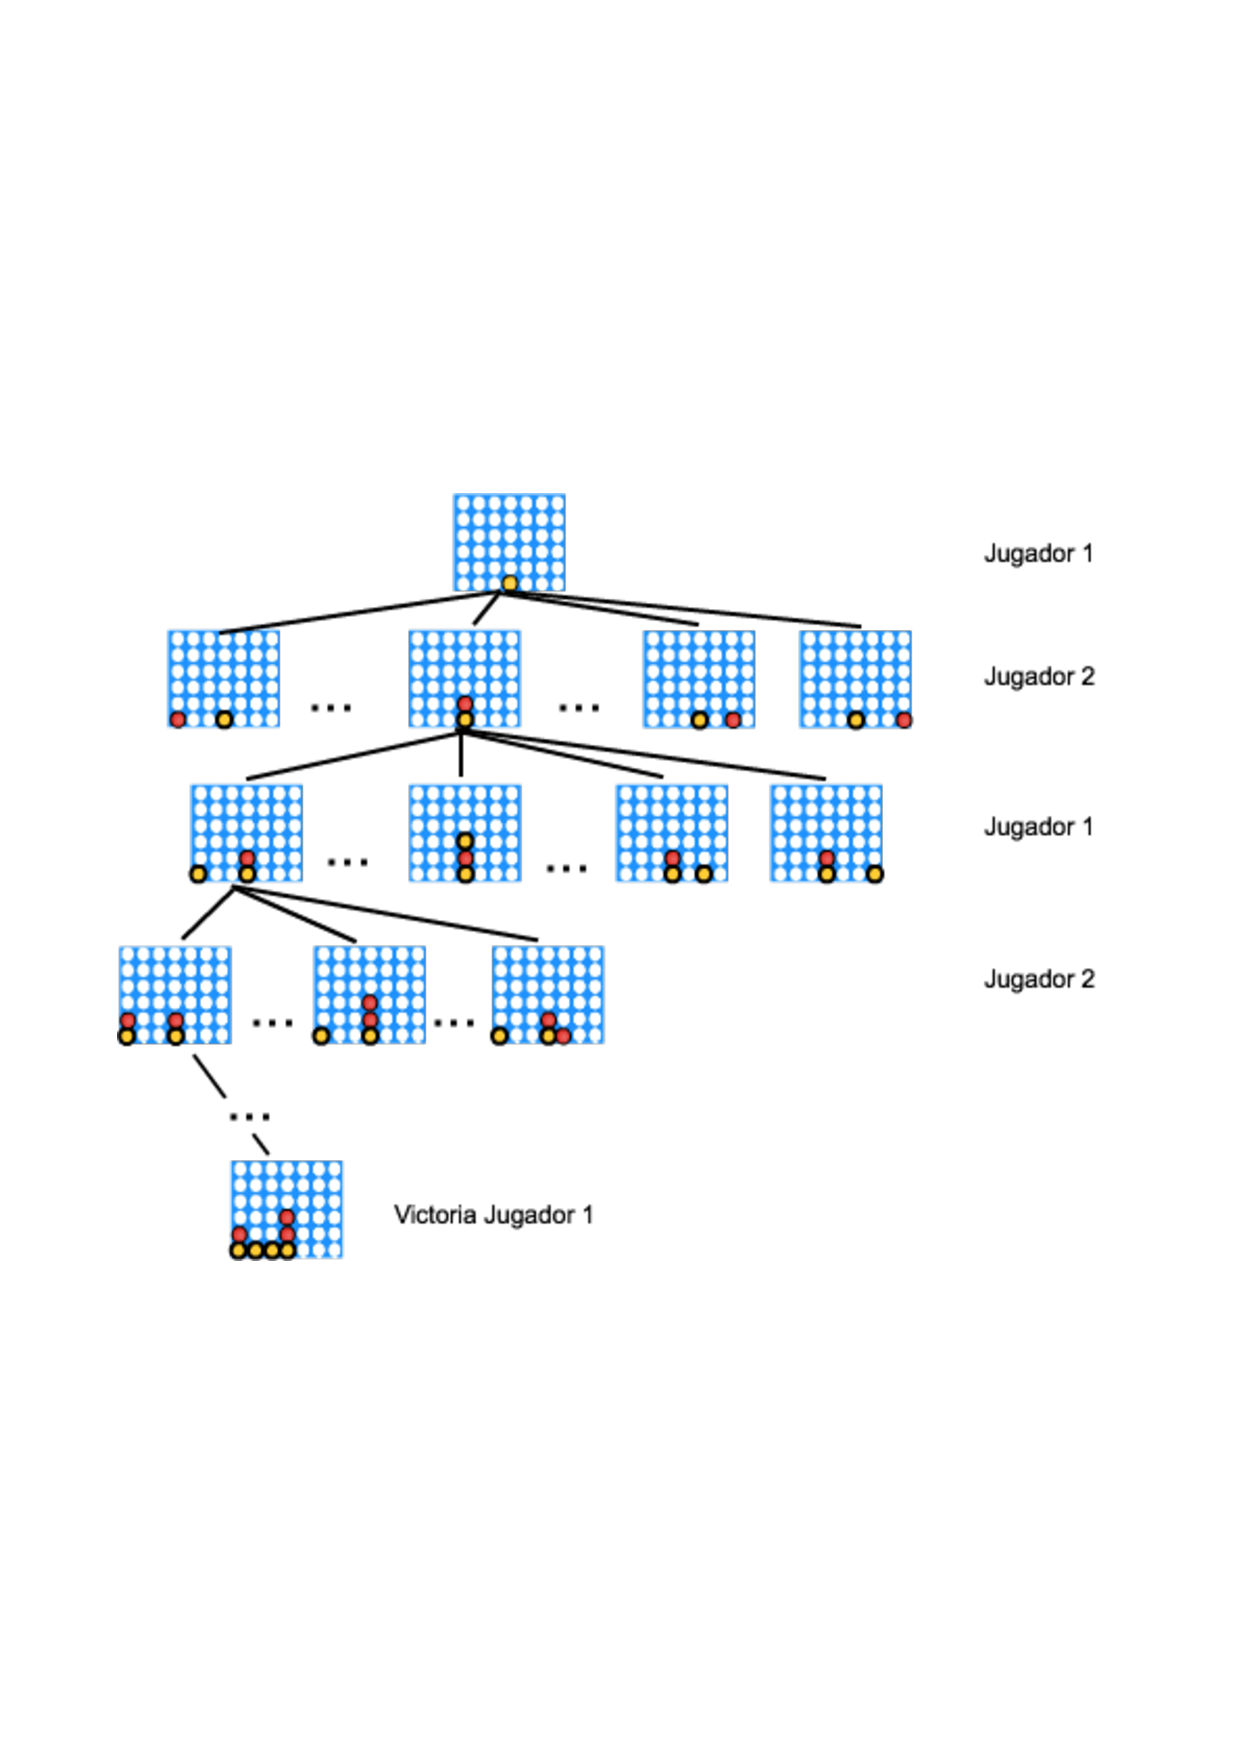
\includegraphics[width=12cm]{connect4-tree-YR}
\caption{Detalle de posibles movimientos en el espacio de soluciones de Conecta 4}
\end{DoxyImage}


El tamaño real de un tablero de Conecta 4 es de 6 filas x 7 columnas, con lo que cada nodo del árbol tiene hasta 7 hijos. Si una columna del tablero estuviera completa, habría menos movimientos posibles y por tanto menos hijos para ese nodo. Los nodos en los que la partida ya está resuelta (por victoria de uno de los jugadores o por no quedar movimientos posibles) serían los nodos hoja del árbol.

De este modo, en el primer nivel del árbol (considerando 1 turno desde el tablero actual), almacenaríamos hasta 7 jugadas posibles o tableros diferentes. En el segundo nivel (considerando 2 turnos desde el actual), almacenaríamos hasta 7$^\wedge$2 tableros posibles. En el tercero, hasta 7$^\wedge$3. Y así sucesivamente. El estudiante debe ser consciente del coste de almacenar y recorrer este volumen de tableros para implementar métricas de recomendación de movimientos que sean viables (coste razonable en tiempo y memoria). Por ejemplo, se recomienda implementar métricas que utilicen un árbol de movimientos para los próximos N turnos desde el tablero actual, donde N queda a elección del estudiante, para acotar el consumo en tiempo y memoria de la implementación de estas métricas.

Además, a medida que el juego va avanzando, se recomienda reutilizar las ramas del árbol de soluciones que siguen siendo posibles y utilizar mecanismos de poda (ya implementados en el T\+DA \hyperlink{classArbolGeneral}{Arbol\+General}) para liberar espacio en memoria eliminando las ramas con movimientos que no se han tomado.

En esta práctica, el estudiante deberá proponer e implementar distintas métricas para guiar la decisión del jugador automático, representando todas las jugadas posibles para los próximos N turnos utilizando un T.\+D.\+A. Árbol General.\hypertarget{index_tareas}{}\subsection{Tareas a realizar}\label{index_tareas}
Se proprocionan\+:
\begin{DoxyEnumerate}
\item T.\+D.\+A. \hyperlink{classTablero}{Tablero}\+: representación del tablero de Conecta 4. Un objeto tablero representa un instante dado de una partida del Conecta 4, es decir, la disposición de las fichas de ambos jugadores sobre el tablero y el turno del jugador al que le corresponde hacer el próximo movimiento.
\item T.\+D.\+A. \hyperlink{classMando}{Mando}\+: representación gráfica del tablero de Conecta 4. Incluye la gestión de Entrada/\+Salida que permite jugar a Conecta 4 de forma interactiva.
\item T.\+D.\+A. \hyperlink{classArbolGeneral}{Arbol\+General}.
\end{DoxyEnumerate}

Se deberán llevar a cabo las siguientes tareas\+:


\begin{DoxyEnumerate}
\item Construir el T.\+D.\+A. Conecta4, que almacena todos los tableros posibles de Conecta 4 generados en los próximos N turnos a partir de un tablero inicial utilizando las clases T.\+D.\+A. \hyperlink{classArbolGeneral}{Arbol\+General} y T.\+D.\+A. \hyperlink{classTablero}{Tablero}.
\item Definir los métodos del T.\+D.\+A. Conecta4 para la solución de los problemas propuestos, en particular, para la implementación de un jugador automático.
\item Probar los módulos con programas test. Se puede usar la S\+TL en todos los módulos excepto en la implementación del T\+DA \hyperlink{classArbolGeneral}{Arbol\+General}.
\end{DoxyEnumerate}

A continuación se detallan los programas que se deberán desarrollar.\hypertarget{index_jugador_automatico}{}\subsection{Implementar un jugador automático}\label{index_jugador_automatico}
Conecta 4 es un juego de estrategia abstracta donde los contrincantes disponen de información perfecta \mbox{[}Conecta4\mbox{]}. Por norma general, el primer jugador tiene más posibilidades de ganar si introduce la primera ficha en la columna central. Si lo hace en las contiguas se puede forzar un empate, mientras que si la mete en las más alejadas del centro su rival puede vencerle con mayor facilidad. Existen libros y webs donde se explican las mejores estrategias para ganar en el Conecta 4, por ejemplo puede consultarse \mbox{[}Allen13\mbox{]}.

El estudiante debe implementar distintas \char`\"{}métricas\char`\"{} que permitan al jugador automático decidir qué movimiento realizar dada una disposición del tablero. Las métricas implementadas analizarán el espacio de soluciones posible a partir del tablero actual para evaluar cuál es el movimiento más beneficioso para el jugador automático (esto es, el movimiento que más aumente las expectativas de ganar la partida). La calidad de estas métricas dependerá, en parte, de la cantidad de información de que dispongan. De este modo, una métrica que sólo considere dos niveles en profundidad a partir del tablero actual (esto es, todos los movimientos posibles del jugador y todas las repuestas inmediatas del rival) tendrá más limitaciones que una métrica que disponga de todo el árbol de soluciones a partir del tablero actual. Evidentemente, la contrapartida es que una métrica que dispone de todo el árbol de soluciones requiere de un alto consumo en memoria y en tiempo de cómputo (según el tamaño del tablero, almacenar todo el árbol de soluciones puede ser directamente inviable). De este modo, se propone diseñar distintas métricas utilizando un árbol de soluciones con N niveles en profundidad a partir del tablero actual, donde N es variable y su elección se deja al estudiante.

El estudiante debe implementar la clase T\+DA Conecta4 utilizando como tipo rep. el T\+DA. \hyperlink{classArbolGeneral}{Arbol\+General} para representar el espacio de soluciones con profundidad N e implementar distintas métricas que, haciendo uso de esta representación del espacio de soluciones, recomienden un movimiento al jugador automático. Anteriormente se ha descrito una posible métrica inicial que sólo requiere explorar un nivel del espacio de soluciones\+: evaluar si alguno de los movimientos posibles para el jugador automático produce directamente un tablero donde el jugador automático consigue 4 en línea (y, por tanto, gana la partida) o evita un 4 en línea del rival (y, por tanto, evita perder la partida). Otra métrica sencilla que requiere explorar todo el árbol de búsqueda hasta profundidad N consiste en hacer recuento de cuántos nodos a profundidad $<$=N son favorables/desfavorables (victorias/empates/derrotas) al jugador automático para cada nodo hijo del tablero actual, de modo que el hijo con mejores métricas indicará el mejor movimiento posible. Otras métricas más sofisticadas podrían explorar este espacio de búsqueda para considerar no sólo victorias o derrotas, sino también recontar el número de secuencias de tres/dos fichas del jugador automático no rodeadas por fichas del rival en cada uno de los tableros.

Es importante destacar que, para aliviar el costo de almacenamiento de las métricas basadas en árboles de búsqueda, una vez realizado un movimiento, el árbol debe podarse para eliminar los nodos asociados a movimientos alternativos que finalmente no fueron tomados. El T\+DA \hyperlink{classArbolGeneral}{Arbol\+General} incluye métodos de poda facilitan esta tarea.

El estudiante tiene libertad para implementar las métricas sugeridas o cualquier otra para guiar los movimientos del jugador automático. La documentación final a entregar debe recoger una descripción completa de cada métrica implementada y una justificación de sus resultados. Se valorará la dificultad para batir al jugador automático guiado por las métricas implementadas por el estudiante.

En la siguiente sección se detalla cómo implementar este programa principal para jugar a Conecta 4.\hypertarget{index_partida}{}\subsection{Implementar una partida de Conecta 4}\label{index_partida}
Se adjunta un programa de ejemplo ({\ttfamily src/conecta4.\+cpp}) que utiliza los T\+DA \hyperlink{classTablero}{Tablero} y T\+DA \hyperlink{classMando}{Mando} para implementar una partida de Conecta 4 interactiva entre dos jugadores (no automáticos). Nótese que este programa va pidiendo por teclado sucesivamente cada movimiento de ambos jugadores, y no hace uso del T\+DA \hyperlink{classArbolGeneral}{Arbol\+General} (no representa el espacio de soluciones posibles para emitir recomendaciones sobre el mejor movimiento o tomar decisiones automáticas).


\begin{DoxyCode}
\textcolor{preprocessor}{#include <iostream>}
\textcolor{preprocessor}{#include <vector>}
\textcolor{preprocessor}{#include <ctime>}
\textcolor{preprocessor}{#include <cstdlib>}
\textcolor{preprocessor}{#include <stdio.h>}
\textcolor{preprocessor}{#include <unistd.h>}
\textcolor{preprocessor}{#include <termio.h>}         \textcolor{comment}{// Linux/Windows users}
\textcolor{comment}{//#include <termios.h>      // Mac OSX users}

\textcolor{preprocessor}{#include "\hyperlink{ArbolGeneral_8h}{ArbolGeneral.h}"}
\textcolor{preprocessor}{#include "\hyperlink{tablero_8h}{tablero.h}"}
\textcolor{preprocessor}{#include "\hyperlink{mando_8h}{mando.h}"}

\textcolor{keyword}{using namespace }\hyperlink{namespacestd}{std};

\textcolor{comment}{// Captura el caracter pulsado por teclado (sin necesidad de pulsar, a continuación, Enter).}
\textcolor{comment}{// Devuelve: Caracter pulsado.}

\textcolor{keywordtype}{char} getch() \{
 ...
\}

\textcolor{comment}{// Imprime en pantalla el tablero completo, con el mando y el jugador.}
\textcolor{comment}{// t : Tablero que se va a imprimir.}
\textcolor{comment}{// m : Mando indicando la posición del jugador.}

\textcolor{keywordtype}{void} imprimeTablero(\hyperlink{classTablero}{Tablero} & t, \hyperlink{classMando}{Mando} & m)\{
    cout << m.\hyperlink{classMando_aaf8c918ecbce5c8173fcf40e04c8b0b7}{GetJugador}() << endl;
    cout << t ;
    cout << m.\hyperlink{classMando_abcc813b0881e56ed976eea2ce6b7fd12}{GetBase}() << endl;
    cout << m.\hyperlink{classMando_a7e02a04343208f949a88e720ba63a281}{GetMando}() << endl;
\}


\textcolor{comment}{// Implementa el desarrollo de una partida de Conecta 4 con dos jugadores humanos}
\textcolor{comment}{// Devuelve: identificador (int) del jugador que gana la partida}
\textcolor{keywordtype}{int} jugar\_partida() \{

    \hyperlink{classTablero}{Tablero} tablero(5, 7);      \textcolor{comment}{//Tablero 5x7}
    \hyperlink{classMando}{Mando} mando(tablero);       \textcolor{comment}{//Mando para controlar E/S de tablero}
    \textcolor{keywordtype}{char} c = 1;
    \textcolor{keywordtype}{int} quienGana = tablero.quienGana();
    \textcolor{comment}{//mientras no haya ganador y no se pulse tecla de terminación}
    \textcolor{keywordflow}{while}(c != \hyperlink{classMando_a3c4e7465d5b25fcaf8f3b50b444421a3}{Mando::KB\_ESCAPE} && quienGana == 0) \{
        system(\textcolor{stringliteral}{"clear"});
        mando.actualizarJuego(c, tablero);  \textcolor{comment}{// actualiza tablero según comando c }
        imprimeTablero(tablero, mando);     \textcolor{comment}{// muestra tablero y mando en pantalla}
        quienGana = tablero.quienGana();    \textcolor{comment}{// hay ganador?}
        \textcolor{keywordflow}{if}(quienGana==0) c = getch();       \textcolor{comment}{// Capturamos la tecla pulsada.    }
    \}

    \textcolor{keywordflow}{return} tablero.quienGana();
\}

\textcolor{keywordtype}{int} main(\textcolor{keywordtype}{int} argc, \textcolor{keywordtype}{char} *argv[])\{
    \textcolor{keywordtype}{int} ganador = jugar\_partida();
    cout << \textcolor{stringliteral}{"Ha ganado el jugador "} << ganador << endl;
\}  
\end{DoxyCode}


El estudiante debe implementar una partida de Conecta 4 en la que uno de los jugadores realiza sus movimientos automáticamente y el otro jugador introduce sus movimientos por teclado. Utilice el código de {\ttfamily src/conecta4.\+cpp} como base para programar este módulo. El programa debe permitir elegir cuál es el jugador que inicia la partida\+: el jugador automático o el humano.

Además, en caso de implementar distintas métricas que guían al jugador automático, el programa contará con un argumento entero que permite identificar la métrica utilizada por el jugador automático (métrica 1, métrica 2, y así sucesivamente). La métrica 1 será, por defecto, la que mejor resultados haya obtenido para el estudiante.

Finalmente, el programa debe también permitir definir el tamaño del tablero.

En resumen, el módulo a desarrollar por el estudiante debe tener los siguientes argumentos\+:

{\ttfamily prompt \%$>$ conecta4 $<$filas\+\_\+tablero$>$ $<$cols\+\_\+tablero$>$ $<$metrica$>$ $<$turno$>$}

Donde\+:


\begin{DoxyItemize}
\item {\ttfamily $<$filas\+\_\+tablero$>$, $<$cols\+\_\+tablero$>$}\+: especifica las dimensiones del tablero (por defecto, 4 en ambas opciones para tablero 4x4)
\item {\ttfamily $<$metrica$>$}\+: indica la métrica a utilizar para guiar al jugador automático. Comenzar a numerar con 1 y en adelante, en orden de mejores a peores resultados obtenidos con esa métrica para el jugador automático. 1 es la opción por defecto (la métrica con mejores resultados). 0 para que la partida se desarrolle entre dos jugadores humanos (sin jugador automático).
\item {\ttfamily $<$turno$>$} indica qué jugador tiene el primer turno\+:
\begin{DoxyItemize}
\item 1\+: primer turno para el jugador humano
\item 2\+: primer turno para el jugador automático
\end{DoxyItemize}
\end{DoxyItemize}\hypertarget{index_ArbolGeneral}{}\subsection{Manejo del T.\+D.\+A. Arbol\+General}\label{index_ArbolGeneral}
Se adjunta un programa de ejemplo ({\ttfamily src/arboltablero\+\_\+test.\+cpp}) en el que se exhibe alguna funcionalidad asociada a los T\+DA \hyperlink{classTablero}{Tablero} y \hyperlink{classArbolGeneral}{Arbol\+General}. En este programa se crean distintos objetos \hyperlink{classTablero}{Tablero} con distintas jugadas posibles de Conecta 4 y una estructura \hyperlink{classArbolGeneral}{Arbol\+General} que almacena jerárquicamente estos tableros.

En particular, se muestra como\+:

Para T\+DA \hyperlink{classTablero}{Tablero}\+:
\begin{DoxyItemize}
\item crear de tableros con las dimensiones deseadas
\item colocar ficha para el jugador que dispone del turno
\item cambiar turno entre jugadores
\end{DoxyItemize}

Para T\+DA \hyperlink{classArbolGeneral}{Arbol\+General}\+:
\begin{DoxyItemize}
\item crear de árboles con T\+DA \hyperlink{classTablero}{Tablero} como nodos
\item obtener el nodo raiz de un \hyperlink{classArbolGeneral}{Arbol\+General}
\item insertar nodos como hijomasizquierda
\item insertar nodos como hermanoderecha
\item imprimir \hyperlink{classArbolGeneral}{Arbol\+General} en preorden
\item podar una rama del \hyperlink{classArbolGeneral}{Arbol\+General}
\end{DoxyItemize}


\begin{DoxyCode}
\textcolor{preprocessor}{#include <iostream>}
\textcolor{preprocessor}{#include "\hyperlink{ArbolGeneral_8h}{ArbolGeneral.h}"}
\textcolor{preprocessor}{#include "\hyperlink{tablero_8h}{tablero.h}"}
\textcolor{preprocessor}{#include <string>}

\textcolor{keyword}{using namespace }\hyperlink{namespacestd}{std};


\textcolor{keywordtype}{int} main(\textcolor{keywordtype}{int} argc, \textcolor{keywordtype}{char} *argv[])\{

  \textcolor{comment}{//Tablero vacío 5x7}
    \hyperlink{classTablero}{Tablero} tablero(5, 7);

    \textcolor{comment}{//Manualmente se insertan algunos movimientos: }
    tablero.colocarFicha(3);  \textcolor{comment}{//Jugador 1 inserta ficha en columna 3}
    tablero.cambiarTurno();
    tablero.colocarFicha(1);  \textcolor{comment}{//Jugador 2 inserta ficha en columna 1}
    tablero.cambiarTurno();
    tablero.colocarFicha(3);  \textcolor{comment}{//Jugador 1 inserta ficha en columna 3.}
    tablero.cambiarTurno();
    
    \textcolor{comment}{//Se muestra el tablero }
    cout << \textcolor{stringliteral}{"Tablero obtenido tras tres movimientos: \(\backslash\)n"}<<tablero; 

    \textcolor{comment}{//A partir de la situación actual del tablero, montamos un árbol para estudiar algunas posibilidades. }

    \textcolor{comment}{// Éste es el árbol que queremos montar: }
    \textcolor{comment}{//        tablero}
    \textcolor{comment}{//          |}
    \textcolor{comment}{//      |---------------|}
    \textcolor{comment}{//    tablero1      tablero2}
    \textcolor{comment}{//                      |}
    \textcolor{comment}{//                  tablero3}


    \textcolor{comment}{//Árbol 'partida', con 'tablero' como nodo raíz}
    \hyperlink{classArbolGeneral}{ArbolGeneral<Tablero>} partida(tablero);

    \textcolor{comment}{//Estudio opciones a partir de tablero: Jugador 2 coloca ficha en columna 1. (tablero1)}
    \hyperlink{classTablero}{Tablero} tablero1(tablero);          \textcolor{comment}{//tablero queda sin modificar}
    tablero1.colocarFicha(1);   
    \hyperlink{classArbolGeneral}{ArbolGeneral<Tablero>} arbol1 (tablero1);  \textcolor{comment}{//creo árbol con un nodo (tablero1)}

    \textcolor{comment}{//Otra opción: Jugador 2 coloca ficha en columna 2. (tablero2)}
    \hyperlink{classTablero}{Tablero} tablero2(tablero);          \textcolor{comment}{//tablero queda sin modificar}
    tablero2.colocarFicha(2);
    \hyperlink{classArbolGeneral}{ArbolGeneral<Tablero>} arbol2(tablero2);   \textcolor{comment}{//creo árbol con un nodo}

    \textcolor{comment}{// Sobre la última opción, ahora contemplo la posibilidad de que }
    \textcolor{comment}{//  Jugador 1 coloque ficha también en columna 2. }
    tablero2.cambiarTurno();          \textcolor{comment}{//modifico tablero2 (esta modificación sería tablero3)}
    tablero2.colocarFicha(2); 
    \hyperlink{classArbolGeneral}{ArbolGeneral<Tablero>} arbol3 (tablero2);  \textcolor{comment}{//creo árbol con un nodo}
    arbol2.insertar\_hijomasizquierda(arbol2.raiz(), arbol3);  \textcolor{comment}{//añado este árbol como hijo de arbol2}

    \textcolor{comment}{// Inserto arbol1 y arbol2 como hijos de partida. }
    \textcolor{comment}{// arbol1 es el hijo más a la izquierda y arbol2 es hermano a la derecha de arbol1}
  
    \textcolor{comment}{//  Forma de hacerlo A: inserto varios hijomasizquierda en el orden inverso al deseado}
    \textcolor{comment}{//  partida.insertar\_hijomasizquierda(partida.raiz(), arbol2);}
    \textcolor{comment}{//  partida.insertar\_hijomasizquierda(partida.raiz(), arbol1);  //hijomasizquierda desplaza al anterior
       a la derecha}
  
    \textcolor{comment}{// Forma de hacerlo B: inserto un hijomasizquierda y hermanoderecha}
    partida.insertar\_hijomasizquierda(partida.raiz(), arbol1);              \textcolor{comment}{//inserto un hijomasizquierda}
    partida.insertar\_hermanoderecha(partida.hijomasizquierda(partida.raiz()), arbol2);  \textcolor{comment}{//le inserto un
       hermanoderecha}
    

    \textcolor{comment}{// Recorremos en preorden para comprobar el arbol 'partida' resultante}
    cout << \textcolor{stringliteral}{"\(\backslash\)nÁrbol en preorden: \(\backslash\)n"}<<endl; 
    partida.recorrer\_preorden();

    \textcolor{comment}{// Podamos el hijomasizquierda y recorremos en preorden: }
    \hyperlink{classArbolGeneral}{ArbolGeneral<Tablero>} rama\_podada;
    partida.\hyperlink{classArbolGeneral_a7f2fa2d9be4af4b7be1c334819a04c39}{podar\_hijomasizquierda}(partida.raiz(), rama\_podada);

    cout << \textcolor{stringliteral}{"\(\backslash\)nRecorrido preorden después de podar hijomasizquierda: \(\backslash\)n"}<<endl; 
    partida.recorrer\_preorden();

    \textcolor{keywordflow}{return} 0;
\}
\end{DoxyCode}


El estudiante deber revisar detenidamente este código y la documentación completa asociada a las clases T\+DA \hyperlink{classTablero}{Tablero} y T\+DA \hyperlink{classArbolGeneral}{Arbol\+General} para familiarizarse con su manejo y sacarles el máximo partido para la implementación del T.\+D.\+A. Conecta4.\hypertarget{index_recomendaciones}{}\subsection{Recomendaciones}\label{index_recomendaciones}

\begin{DoxyItemize}
\item Analice con detenimiento la documentación de las clases proporcionadas\+: T.\+D.\+A. \hyperlink{classArbolGeneral}{Arbol\+General}, T.\+D.\+A. \hyperlink{classTablero}{Tablero} y T.\+D.\+A. \hyperlink{classMando}{Mando}. Parte importante del esfuerzo que debe realizar en esta práctica es entender cómo debe utilizar estas clases para su proyecto. Esta práctica es habitual en empresas\+: para el desarrollo de un proyecto se cuenta con parte del código desarrollado previamente por otro equipo.
\item Para acotar el espacio de búsqueda y el tamaño de los objetos \hyperlink{classArbolGeneral}{Arbol\+General}, comience el desarrollo de su proyecto considerando tableros más pequeños (por ejemplo, 4x4). Cuando el funcionamiento sea correcto, amplíe progresivamente el tamaño de los tableros. Del mismo modo, considere con cautela la profundidad máxima N que va a explorar en el árbol de soluciones. Comience con un valor bajo de N y estudie hasta qué valor de N (depende del tamaño del tablero) es viable el cálculo de sus métricas.
\end{DoxyItemize}\hypertarget{index_entrega}{}\subsection{Entrega}\label{index_entrega}
El estudiante deberá empaquetar todos los archivos relacionados en el proyecto en un archivo con nombre “conecta4.\+tgz” y entregarlo antes de la fecha que se publicará en la página web de la asignatura. Tenga en cuenta que no se incluirán ficheros objeto, ni ejecutables, ni la carpeta datos. Es recomendable que haga una “limpieza” para eliminar los archivos temporales o que se puedan generar a partir de los fuentes. El estudiante debe incluir el archivo Makefile para realizar la compilación. Tenga en cuenta que los archivos deben estar distribuidos en directorios\+:

conecta4
\begin{DoxyItemize}
\item Makefile
\item include -- Carpeta con ficheros de cabecera (.h)
\item src --Carpeta con código fuente (.cpp)
\item doc --Carpeta con Documentación
\item obj -- Carpeta para código objeto (.o)
\item bin -- Carpeta para ejecutables
\item datos -- Carpeta para ficheros de datos
\end{DoxyItemize}

Para realizar la entrega, en primer lugar, realice la limpieza de archivos que no se incluirán en ella, y sitúese en la carpeta superior (en el mismo nivel de la carpeta \char`\"{}conecta4\char`\"{}) para ejecutar\+: 
\begin{DoxyCode}
prompt% tar zcv conecta4.tgz conecta4
\end{DoxyCode}
 tras lo cual, dispondrá de un nuevo archivo conecta4.\+tgz que contiene la carpeta conecta4 así como todas las carpetas y archivos que cuelgan de ella.

La fecha límite de entrega es el día 22 de Enero de 2017 a las 23\+:59.\hypertarget{index_referencias}{}\subsection{Referencias}\label{index_referencias}
\mbox{[}Allen13\mbox{]} James D. Allen. \char`\"{}\+Expert Play in Connect-\/\+Four\char`\"{} (en inglés). Archivado desde el original el 4 de noviembre de 2015. \href{http://web.archive.org/web/20141125065033/http://homepages.cwi.nl/~tromp/c4.html}{\tt http\+://web.\+archive.\+org/web/20141125065033/http\+://homepages.\+cwi.\+nl/$\sim$tromp/c4.\+html}

\mbox{[}Conecta4\mbox{]} \href{https://es.wikipedia.org/wiki/Conecta_4}{\tt https\+://es.\+wikipedia.\+org/wiki/\+Conecta\+\_\+4}

\mbox{[}G\+A\+R06b\mbox{]} Garrido, A. Fdez-\/\+Valdivia, J. \char`\"{}\+Abstracción y estructuras de datos en C++\char`\"{}. Delta publicaciones, 2006. 